\begin{figure}[!htbp]
\begin{center}

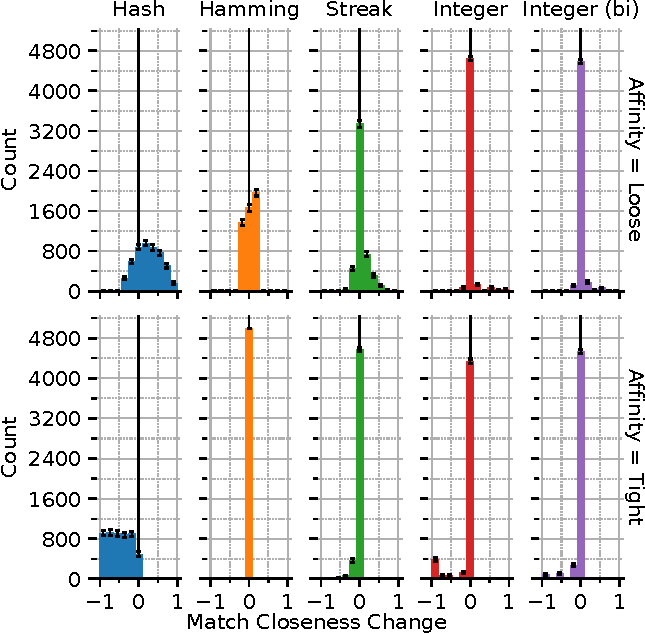
\includegraphics[width=\columnwidth]{img/mutational_step/bitweight=0dot5+seed=1+title=low-mutational-step+viz=hist+_data_hathash_hash=95a57768de56995a+_script_fullcat_hash=aa068ad24b386169+ext=}
\caption{
Distributions of mutation effects on match distance for loosely matched (pre-mutation match distance $> 0.5$) and tightly matched (pre-mutation match distance $< 0.01$) tag pairs.
Note that match closeness change (rather than mast distance change) is plotted so that better-matching mutational outcomes fall to the right and worse-matching mutational outcomes fall to the left.
Error bars are 95\% confidence intervals calculated using the Wilson score method with continuity correction \citep{newcombe1998two}.
Supplementary Figure \ref{fig:mutational_step_supp} shows the cumulative distribution of all sampled match distance changes for each metric.
}
\label{fig:mutational_step}

\end{center}
\end{figure}
